\documentclass[11pt]{article}

\pdfminorversion=4

% use packages
\usepackage[utf8]{inputenc}
\usepackage{amsmath}
\usepackage{amsthm}
\usepackage{amsfonts}
\usepackage{amscd}
\usepackage{amssymb}
\usepackage{natbib}
\usepackage{url}
\usepackage[table,xcdraw,usenames]{xcolor}
%\usepackage[usenames]{color}

\usepackage{graphicx}
\usepackage{subcaption}
\usepackage{mathtools}
\usepackage{enumitem}
\usepackage{authblk}
\usepackage{bm}
\usepackage{comment}
\usepackage{pdfpages}

\usepackage{hyperref}
\usepackage{caption}
\usepackage{float}
%\usepackage[caption = false]{subfig}
\usepackage{tikz}
\usepackage{multirow}
\usepackage[linesnumbered, ruled,vlined]{algorithm2e}
\usepackage{pdflscape}
\usepackage{etoolbox}

%\AtBeginEnvironment{align}{\setcounter{equation}{0}} % https://tex.stackexchange.com/questions/349247/how-do-i-reset-the-counter-in-align

% margin setup
\usepackage{geometry}
\geometry{margin=0.8in}

% function definition
\newcommand{\V}{\textbf{V}}
\newcommand{\weight}{\pi}
\newcommand{\ret}{\textbf{r}}
\newcommand{\y}{\textbf{y}}
\newcommand{\w}{\textbf{w}}
\newcommand{\x}{\textbf{x}}
\newcommand{\dbf}{\textbf{d}}
\newcommand{\X}{\textbf{X}}
\newcommand{\Y}{\textbf{Y}}
%\newcommand{\L}{\textbf{L}}
\newcommand{\Hist}{\mathcal{H}}
\newcommand{\Prob}{\mathbb{P}}
\def\mbf#1{\mathbf{#1}} % bold but not italic
\def\ind#1{\mathrm{1}(#1)} % indicator function
\newcommand{\simiid}{\stackrel{iid}{\sim}} %[] IID 
\def\where{\text{ where }} % where
\newcommand{\indep}{\perp \!\!\! \perp } % independent symbols
\def\cov#1#2{\mathrm{Cov}(#1, #2)} % covariance 
\def\mrm#1{\mathrm{#1}} % remove math
\newcommand{\reals}{\mathbb{R}} % Real number symbol
\def\t#1{\tilde{#1}} % tilde
\def\normal#1#2{\mathcal{N}(#1,#2)} % normal
\def\mbi#1{\boldsymbol{#1}} % Bold and italic (math bold italic)
\def\v#1{\mbi{#1}} % Vector notation
\def\mc#1{\mathcal{#1}} % mathical
\DeclareMathOperator*{\argmax}{arg\,max} % arg max
\DeclareMathOperator*{\argmin}{arg\,min} % arg min
\def\E{\mathbb{E}} % Expectation symbol
\def\mc#1{\mathcal{#1}}
\def\var#1{\mathrm{Var}(#1)} % Variance symbol
\def\checkmark{\tikz\fill[scale=0.4](0,.35) -- (.25,0) -- (1,.7) -- (.25,.15) -- cycle;} % checkmark
\newcommand\red[1]{{\color{red}#1}}
\def\bs#1{\boldsymbol{#1}}
\def\P{\mathbb{P}}
\def\var{\mathbf{Var}}
\def\naturals{\mathbb{N}}
\def\cp{\overset{p}{\to}}
\def\clt{\overset{\mathcal{L}^2}{\to}}

\setcounter{tocdepth}{4}
\setcounter{secnumdepth}{4}

\newtheorem{corollary}{Corollary}
\newcommand{\ceil}[1]{\lceil #1 \rceil}
\newcommand{\norm}[1]{\left\lVert#1\right\rVert} % A norm with 1 argument
\DeclareMathOperator{\Var}{Var} % Variance symbol

\newtheorem{cor}{Corollary}
\newtheorem{lem}{Lemma}
\newtheorem{thm}{Theorem}
\newtheorem{defn}{Definition}
\newtheorem{prop}{Proposition}
\theoremstyle{definition}
\newtheorem{remark}{Remark}
\hypersetup{
  linkcolor  = blue,
  citecolor  = blue,
  urlcolor   = blue,
  colorlinks = true,
} % color setup

% proof to proposition 
\newenvironment{proof-of-proposition}[1][{}]{\noindent{\bf
    Proof of Proposition {#1}}
  \hspace*{.5em}}{\qed\bigskip\\}
% general proof of corollary
  \newenvironment{proof-of-corollary}[1][{}]{\noindent{\bf
    Proof of Corollary {#1}}
  \hspace*{.5em}}{\qed\bigskip\\}
% general proof of lemma
  \newenvironment{proof-of-lemma}[1][{}]{\noindent{\bf
    Proof of Lemma {#1}}
  \hspace*{.5em}}{\qed\bigskip\\}

\allowdisplaybreaks

\title{Forecast Adjustment Under Shocks: A Unification}
\author{David P. Lundquist\thanks{davidl11@ilinois.edu}, Daniel J. Eck\thanks{dje13@illinois.edu} }
\affil{Department of Statistics, University of Illinois at Urbana-Champaign}
\date{\today}

\begin{document}

\maketitle

\begin{abstract} 
Structural shocks to time series may give an observer reason to doubt the credibility of the default forecasting function.  This work systematizes and unifies the rich landscape of model adjustment and model correction methods, with a special focus on forecast adjustment under the presence of shocks.  We demonstrate the usefulness of similarity-based methods in forecasting and present several specific models that can benefit, along with formal results for some of those special cases.

\end{abstract}





\section{Introduction}\label{Introduction}

\textbf{Plan}

What the paper should do
\begin{itemize}
  \item Introduce an existing diffuse set of approaches to adjusting forecasts (\ref{Introduction})
  \item Explain when/how similarity can help us forecast. \ref{meaning_use}
  \item distinguish the method from various tools that inspired it (\ref{Introduction})
  \item show a few special cases, both examples and formal results (\ref{special_cases})
  \item discuss limitations of the method (\ref{Limitations})
  \item propose extensions (\ref{Extensions})
\end{itemize}

What the paper should NOT do

\begin{itemize}
  \item Wade too deeply into distance-based weighting details.  We can refer to other work?
  \item wade too deeply into any of the special cases
  \item Tackle non-scalar random quantities (density forecasts, etc)
  \item Forecast combination

\end{itemize}

For various modeling and prediction tasks in time series and panel data, the salient challenge is not predicting when an event will occur but what its key properties will be.  In the familiar case of scalar time series, those properties can include its post-event direction, moments, sign, magnitude, duration, and correlation structure, all over an arbitrary horizon or perhaps multiple horizons. This is not to say that predicting the arrival of an event is easy. In some cases, it may be difficult or impossible, and therefore preparing for an antipicated shock is the best one can hope for.

This work focuses on model adjustment amid structual shocks that undermine the reliability of the  model at hand.  Forecasting under anticipated shocks raises unavoidable questions: should the forecast model be abandoned in favor of a discretionary or ad-hoc or one-off adjustment?  Does the does the discretion of a forecaster rule out a quantitative method for making the adjustment?  What is the ultimate purpose of the adjustment, and how it is to be used?  For how long is the adjustment necessary or reliable?

Herein we systematize and unify a range of conceptual approaches and tools that have developed across the broad ecosystem of the econometric and forecasting literatures.  Additionally, we delineate a specific type of forecasting task called post-shock forecasting, which we broadly define as forecasting under a known shock.

Forecast model adjustment, known most widely perhaps by the term intercept-correction, has received the most attention in several articles and book chapters \citep{hendry1994theory,clements1996intercept,clements1998forecasting}.  Of special importance is the distinction between discretionary and automated intercepts corrections. \cite{hendry1994theory} define scalar intercept corrections to be automated when they follow the simple rule of adding an estimation residual $e_{t}$ to subsequent (possibly but not necessarily all) forecasts $\hat f_{t+1},\hat f_{t+2},...$.  This procedure can colloquially referred to as setting the model back on track \citep{hendry1994theory}.  In \cite{hendry1994theory}, after recounting the bipartite division of interception corrections in discretionary and automated varieties, the authors present a six-way taxonomy of information that a modeler possesses at the time a forecast is made.  The authors also consider structural change in the data-generating process during the forecast period, including as early as the first point in the forecast period (specifically in the autoregressive structure), as well as what is for them the more interesting case: structural change between $T^{*}-1$ and $T^{*}$.  This current work finds both cases interesting.  What if we could predict well the intercept shift that occurs between $T^{*}$ and $T^{*}+1$?

Post-shock forecasting procedures have been explored in \cite{lin2021minimizing,lundquist2024volatility}, where the AR(1) and GARCH($m,s$) cases, respectively, are treated.  Both works target additive parameters in scalar time series, predicting those random effects by aggegating information from other time series.  The authors leave several stones unturned, including a more general, dare say comprehensive treatment of how to forecast under any sort of shock.

A practitioner interested in forecast adjustment can choose between procedures that discretionary or automated, a variety of choices for the collection of data assembled to perform the correction, whether the data is internal (i.e. from the time series itself) or external, the parametric term to be corrected (e.g. intercept, coefficients), if any, as well as the correction function (i.e. the mapping from the data to the corrective term), including the weighting applied to the assembled data (e.g. Nearest-Neighbor, arithmetic mean, kernel methods).

The procedure presented herein is a discretionary procedure for intercept correction that integrates data internal or external to the time series under study in a systematic manner.  The correction function uses an optimization step inspired by the causal inference literature.  Outside of \citet{lin2021minimizing,lundquist2024volatility}, we are not aware of prior work that both introduces a parametric specification for nonzero errors and introduces a procedure for weighting appropriately the nonzero errors of similar shocks occurring outside the time series under study.  We are also not familiar with any prior work that attempts to account for anticipated nonzero errors using an a parametric adjustment, i.e., a ``correction function''.  

\subsection{Motivation for Intercept Correction}

\subsubsection{Setting levels back on track}

\subsubsection{Mismeasured data}

Mismeasured data is discussed in \cite[p. 166]{hendry1994theory} as a motivator for intercept correction.  Could similarity-based correction help?  Here is an idea: if we believe that our most recent measurement of the series is noisy, we can disregard the point itself and instead take a convex combination of that point and the \cite{lin2021minimizing}-style prediction based on aggregation.

Quinton-Guerrera and Zhong \cite{guerron2017macroeconomic} - concerned with correcting $\beta$ using similarity\\

\subsubsection{Motivation from model evaluation}

Part of the reason for correcting a model springs from the way we evaluate model performance.
Evaluating a Model by Forecast Performance \cite{clements2005evaluating}
\begin{enumerate}

  \item   unconditional versus conditional, models;
  \item internal versus external standards;
  \item checking constancy versus adventitious significance;
  \item ex ante versus ex post evaluation (skip this one?);
  \item 1-step versus multi-horizon forecasts -- this is a relevant question to ask in the context of post-shocking forecasting: should we correct the earliest forecast and then allow the shock to propagate, or should we just correct each term in the horizon, h=1, 2,..., H?
  \item in-sample fixed coefficients versus continuous updating
\end{enumerate}

Here is the argument: if we are going to judge a model by forecast performance, we need to entertain the possibility that the model may breakdown and that our pre-breakdown-based criteria for model performance will be invalidated.

\subsection{The Meaning and Use of Similarity}\label{meaning_use}
Hume? Cite Israeli authors, if so.\\

The notion of similarity appears in various statistical contexts, including matching, synthetic control, nearest-neighbor methods, not to mention the massive area of approximation theory.\\

Similar, in the strong sense, could mean that a shared DGP exists.\\

\textbf{Quantitative} ways of determining similarity\\

Distance function\\

Asymmetric distance functions are useful when we want to explore differences between donors and weight different contributors to that function differently.\\

What about \textbf{qualitative} ways of determining similarity -- \cite{lundquist2024volatility} donors are identified qualitatively

\section{Setting}\label{Section}


In order to motivate our procedure, we provide a visual illustration.  In Figure [decide on which figure to include] %\ref{fig:motivating_piece_convex_combination}, 
we show how the aggregation of estimated excess volatilities from donors in the donor pool works when the correction function is a specially-chosen convex combination of fixed effects from the donor pool.  Our method assumes a credible, parsimonious parameterization in which the shock is an affine transformation of several key covariates.  The key intuition behind this shock parameterization is that as the strength of the linear signal increases relative to the idiosyncratic error, the GARCH estimation of these effects increases in accuracy.  From this, it follows that the aggregated shock estimate increases in accuracy.


\subsection{Model setup}
\label{modelsetup}

In this section, we will to some extent mimick the layout of the other paper.

Assume a researcher has multivariate time series data $\y_{i,t} = (r_{i,t}$, $\x_{i,t}$), $t = 1,$ $\ldots,  T_i$, $i = 1, \ldots, n+1$, and  $\x_{i,t}$ is a vector of covariates such that $\x_{i,t}|\mathcal{F}_{i,t-1}$ is deterministic.  Suppose that the analyst is interested in forecasting the volatility of $r_{1,t}$, the first time series in the collection, which we will denote the time series under study.  We require that each time series $\y_{i,t}$ is subject to a news event following $T^*_i \leq T_{i} + 1$ and before witnessing $T^*_i+1$.  

\begin{align*}
&y_{i,t} = F(\mathcal{F}_{t-1}) + \epsilon_{t}\\
\end{align*}
Let $I(\cdot)$ be an indicator function.  Let $T_i$ denote the time length of the time series $i$ for $i = 1, \ldots, n+1$, and let $T_i^*$ denote the largest time index prior to the arrival of the news shock, with $T_i^* < T_i$.  Let $\delta, \x_{i,t} \in \mathbb{R}^{p}$.  For $t= 1, \ldots, T_i$ and $i = 1, \ldots, n+1$, the model $\mc{M}_1$ is defined as 
\begin{align*}
  \mc{M}_1 \colon \begin{array}{l}
     \sigma^{2}_{i,t} = \omega_{i} + \omega^{*}_{i,t} + \sum^{m_{i}}_{k=1}\alpha_{i,k}a^{2}_{i,t-k} + \sum_{j=1}^{s_{i}}\beta_{i,j}\sigma_{i,t-j}^{2} + \gamma_{i}^{T} \x_{i,t} \text{ }\\[.2cm]
     a_{i,t} = \sigma_{i,t}((1-D^{return}_{i,t})\epsilon_{i,t} + D^{return}_{i,t}\epsilon^{*}_{i})\\[.2cm]
    \omega_{i,t}^{*} = D^{vol}_{i,t}[\mu_{\omega^{*}}+\delta'\x_{i,t}+ u_{i,t}],
  \end{array}
  \end{align*}
with error structure

  \begin{align*}
    \epsilon_{i,t} &\simiid \mc{F}_{\epsilon} \text{ with }  \; \mrm{E}_{\mc{F}_{\epsilon}}(\epsilon) = 0, \mrm{Var}_{\mc{F}_{\epsilon}}(\epsilon)  = 1  \\
    \epsilon^{*}_{i,t} &\simiid \mc{F}_{\epsilon^{*}} \text{ with }  \; \mrm{E}_{\mc{F}_{\epsilon^{*}}}(\epsilon) = \mu_{\epsilon^{*}}, \mrm{Var}_{\mc{F}_{\epsilon^{*}}}(\epsilon^{*})  = \sigma^2_{\epsilon^{*}}  \\
    u_{i,t} & \simiid  \mc{F}_{u} \text{ with }  \; \mrm{E}_{\mc{F}_{u}}(u) = 0, \mrm{Var}_{\mc{F}_{u}}(u) = \sigma^2_{u}\\
    \epsilon_{i,t} & \indep  \epsilon^{*}_{i,t}  \indep u_{i,t}
    \end{align*}
 
    Note that $\mc{M}_{0}$ assumes that $\omega^{*}_i$ have no dependence on the covariates and are i.i.d. with $\E[ \omega^{*}_i]=\mu_{\omega^{*}}$.  


\section{Model Adjustment Using Similarity-Based Parameter Correction: A Global Overview}

In this section, we introduce and discuss a particular approach to model adjustment that is motivated by the circumstances laid out in Section \ref{Section}.
\begin{enumerate}
  \item a random object to forecast that depends on a linear specification or a specification that can be linearized
  \item a parametric model family shared by donors\footnote{Emphasize that there is a non-parametric version of the above: for example, one can use LSTM to predict each of the donor shocks, and then the residuals (or transformations of those residuals, e.g. to percentages) of those n models can be weighted to arrive at a correction term.}
  \item a correction term for the model family shared by donors
  \item a parametric specification for the correction term\\
  
This is important because without a parametric specification that produces fixed effects estimates, we cannot get key scalars to take a convex combination of.\\

Does it draw on data internal or external to the time series under study, or does it draw upon both?

  \item a reliable estimation procedure for the shared model. \\
  
  When we use fixed effect estimation (under ordinary assumptions), we can construct confidence intervals for the fixed effect estimates, and then assuming independence, we can get confidence intervals for convex combinations of fixed effect estimates.
  

  \begin{enumerate}
  \item This should be straightforward
  \end{enumerate}
  \item a reliable estimation procedure for the correction term 
  \begin{enumerate}
    \item This might not be straightforward.  Some models like GARCH, for example, might deliver very noisy estimates for indicator variables that occur just once.
    \item When will it be as simple as a fixed effect?
    \item When will it be something besides a fixed effect?
    \end{enumerate}
  \item a correction function, based on the correction term, that aggregates (i.e. maps) donor correction terms based on some notion of similarity
\end{enumerate}

\section{Methodology for Similarity-based Parameter Correction}

\subsection{Forecasting}

So far we have presented a setting and a data generating process for which we intend to furnish a statistical method.  Now, we present two forecasts for the time series, the latter of which benefits from the proposed method.  In particular, we present the GARCH forecast, also called the \textit{unadjusted} forecast, as well as the \textit{adjusted} forecast, which differs by an additive term:

\begin{align*}
  \text{Forecast 1: } & \hat\sigma^{2}_{unadjusted} = \hat\E[\sigma^{2}_{1,T_{1}^{*}+1}|\mathcal{F}_{T^{*}}] && = && \hat\omega_{i} + \sum^{m_{i}}_{k=1}\hat\alpha_{i,k}a^{2}_{i,t-k} + \sum_{j=1}^{s_{i}}\hat\beta_{i,j}\sigma_{i,t-j}^{2} + \hat\gamma_{i}^{T} \x_{i,t}\\
  \text{Forecast 2: } & \hat\sigma^{2}_{adjusted} = \hat\E[\sigma^{2}_{1,T_{1}^{*}+1}|\mathcal{F}_{T^{*}}] + \hat\omega^{*} && = && \hat\omega_{i} + \sum^{m_{i}}_{k=1}\hat\alpha_{i,k}a^{2}_{i,t-k} + \sum_{j=1}^{s_{i}}\hat\beta_{i,j}\sigma_{i,t-j}^{2} + \hat\gamma_{i}^{T} \x_{i,t} + \hat\omega^{*} \text{ .}
\end{align*}

\subsection{Shock Estimators}
    \label{Shock_Estimators}
   
    The problem of aggregating estimated donor shocks begins with the data constraints.  Taking the estimated shocks as a given, we essentially observe the pair $(\{\hat\omega^{*}_{i}\}^{n+1}_{i=2},\{\textbf{v}_{i}\}^{n+1}_{i=2})$.  We wish to recover weights $\{\weight_{i}\}^{n+1}_{i=2} \in \Delta^{n}$ leading to favorable forecasting properties.  These weights are used to compute $\hat\omega^{*} \coloneq \sum^{n+1}_{i=2}\weight_{i}\hat\omega^{*}_{i}$, our forecast adjustment term.  Since the weights $\{\weight_{i}\}_{i=2}^{n+1}$ are computed using $\mathcal{F}_{T^{*}_{i}}$, the set $\{\weight_{i}\}_{i=2}^{n+1}$ is deterministic, $\textit{modulo}$ any stochastic ingredient in the numerical methods employed to approximate $\x_{1,T^{*}}$ using a convex combination of donor covariates.  We say more about the properties of $\omega^{*}_{i}$ in section $\ref{SVF_properties}$. 

    Following \citet{abadie2003economic,abadie2010synthetic}, let $\|\cdot\|_{\textbf{S}}$ denote any semi-norm on $\mathbb{R}^{p}$, and define

    \begin{align*}
    \{\pi\}_{i=2}^{n+1} = \argmin_{\pi}\|\textbf{v}_{1} - \V_{t}\pi \|_{\textbf{S}} \text{ .}
    \end{align*}
    
\subsection{How is the proposed method distinct from existing tools?}

\subsection{Relaxation of Assumptions}
\subsubsection{How important is a shared DGP?}

\subsection{We can use the method on latent time series}
See \cite{lundquist2024volatility}

\section{Formal Properties and Model-Specific Considerations}\label{special_cases}

 


\subsection{ARIMA}
\cite{lin2021minimizing}
\subsection{GARCH}
We briefly highlight the findings of \citep{lundquist2024volatility}.
\subsection{HAR}
\begin{figure}[h!]
  \begin{center}
    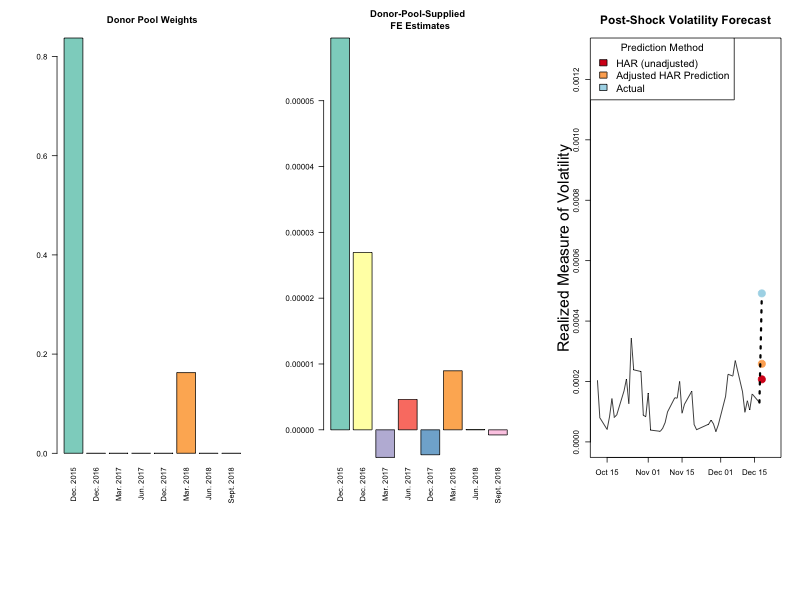
\includegraphics[scale=.4]{real_data_output_plots/savetime_SatJun151644072024__^VIX-^IRX-^XAU_^VIX_2018-12-18-2015-12-15-2016-12-13-2017-03-14-2017-06-13-2017-12-12-2018-03-20-2018-06-12-2018-09-25.png}
    \caption{Volatility series of six i.i.d. GARCH processes, each of which experiences a volatility shock, indicated with a red vertical line, at a uniformly distributed point in the set $\{756,...,2520\}$ of trading days, corresponding to between 3 and 10 years of daily trading data.}
    \label{fig:six_plots}
    \end{center}
  \end{figure}

\subsection{VAR}
Many time series, especially macroeconomic time series, naturally arise as constituents of groups of dependent variables that interact across time.
\subsection{LSTM/GRU}

Here we demonstrate the tremendous capaciousness of our method by applying it to predictions generated by a pair of non-parametric forecasting functions, Long Short Term Memory and GRU.  We will re-examine an application found in \cite{lin2021minimizing}.

We borrow code from\cite{Brownlee_2022}

\begin{itemize}
  % \item \href{https://www.r-bloggers.com/2021/04/lstm-network-in-r/#google_vignette}{a}
  % \item \href{https://sharmasaravanan.medium.com/an-implementation-guide-for-lstm-in-r-2347e4118a2c}{b}
  % \item \href{https://search.r-project.org/CRAN/refmans/TSdeeplearning/html/GRU_ts.html}{c}
  % \item \href{https://medium.com/codex/time-series-prediction-using-lstm-in-python-19b1187f580f#:~:text=In%20conclusion%2C%20LSTM%20models%20are,in%20your%20data%20science%20toolkit.}{d}
  \item \href{https://machinelearningmastery.com/time-series-prediction-lstm-recurrent-neural-networks-python-keras/}{LSTM in Python}
\end{itemize}

\subsection{What are the downsides of aggregating residuals as opposed to aggregating fixed effect estimates?}

Cases:
\begin{enumerate}
  \item Fixed effect is estimated with accuracy 
  \item Fixed effect is estimated with considerable noise.  Hence, the idiosyncratic error is estimated with considerable noise.
  \item idiosyncratic error large
  \item idiosyncratic error small
\end{enumerate}  


\section{Real Data Examples}
This section might not be necessary.
g\section{Discussion}

Are there any situations where we would want to intercept-correct using the post-shock term from \cite{lin2021minimizing} rather than the actual residual?

The forecast horizon --- does it matter?  If so, how so?  \cite{lin2021minimizing} has a one-period horizon.  \cite{clements1998forecasting}{p. 203} discuss how long to keep the forecast adjustment in place.  For a corrected ``slope parameter'', the effect of $h$ is not so clear.\\



\subsection{Extensions}\label{Extensions}
bias-variance tradeoff and MSE decomposition\\

\begin{itemize}
  \item Binary Outcome Forecasts
  \item Density Forecasts
  \item Quantile Forecasts
\end{itemize}

\subsection{Limitations}\label{Limitations}

\subsection{Forecast Combination}
what we are talking about here is not forecast combination, but there may be, nevertheless, a role for forecast combination: combining the forecasts generated by small differences in covariate and/or donor choice, as is done in \cite{lundquist2024volatility}. \\

\clearpage

\bibliographystyle{plainnat}
\bibliography{synthVolForecast}
 
\end{document}